\begin{figure*}[t]
  \centering
  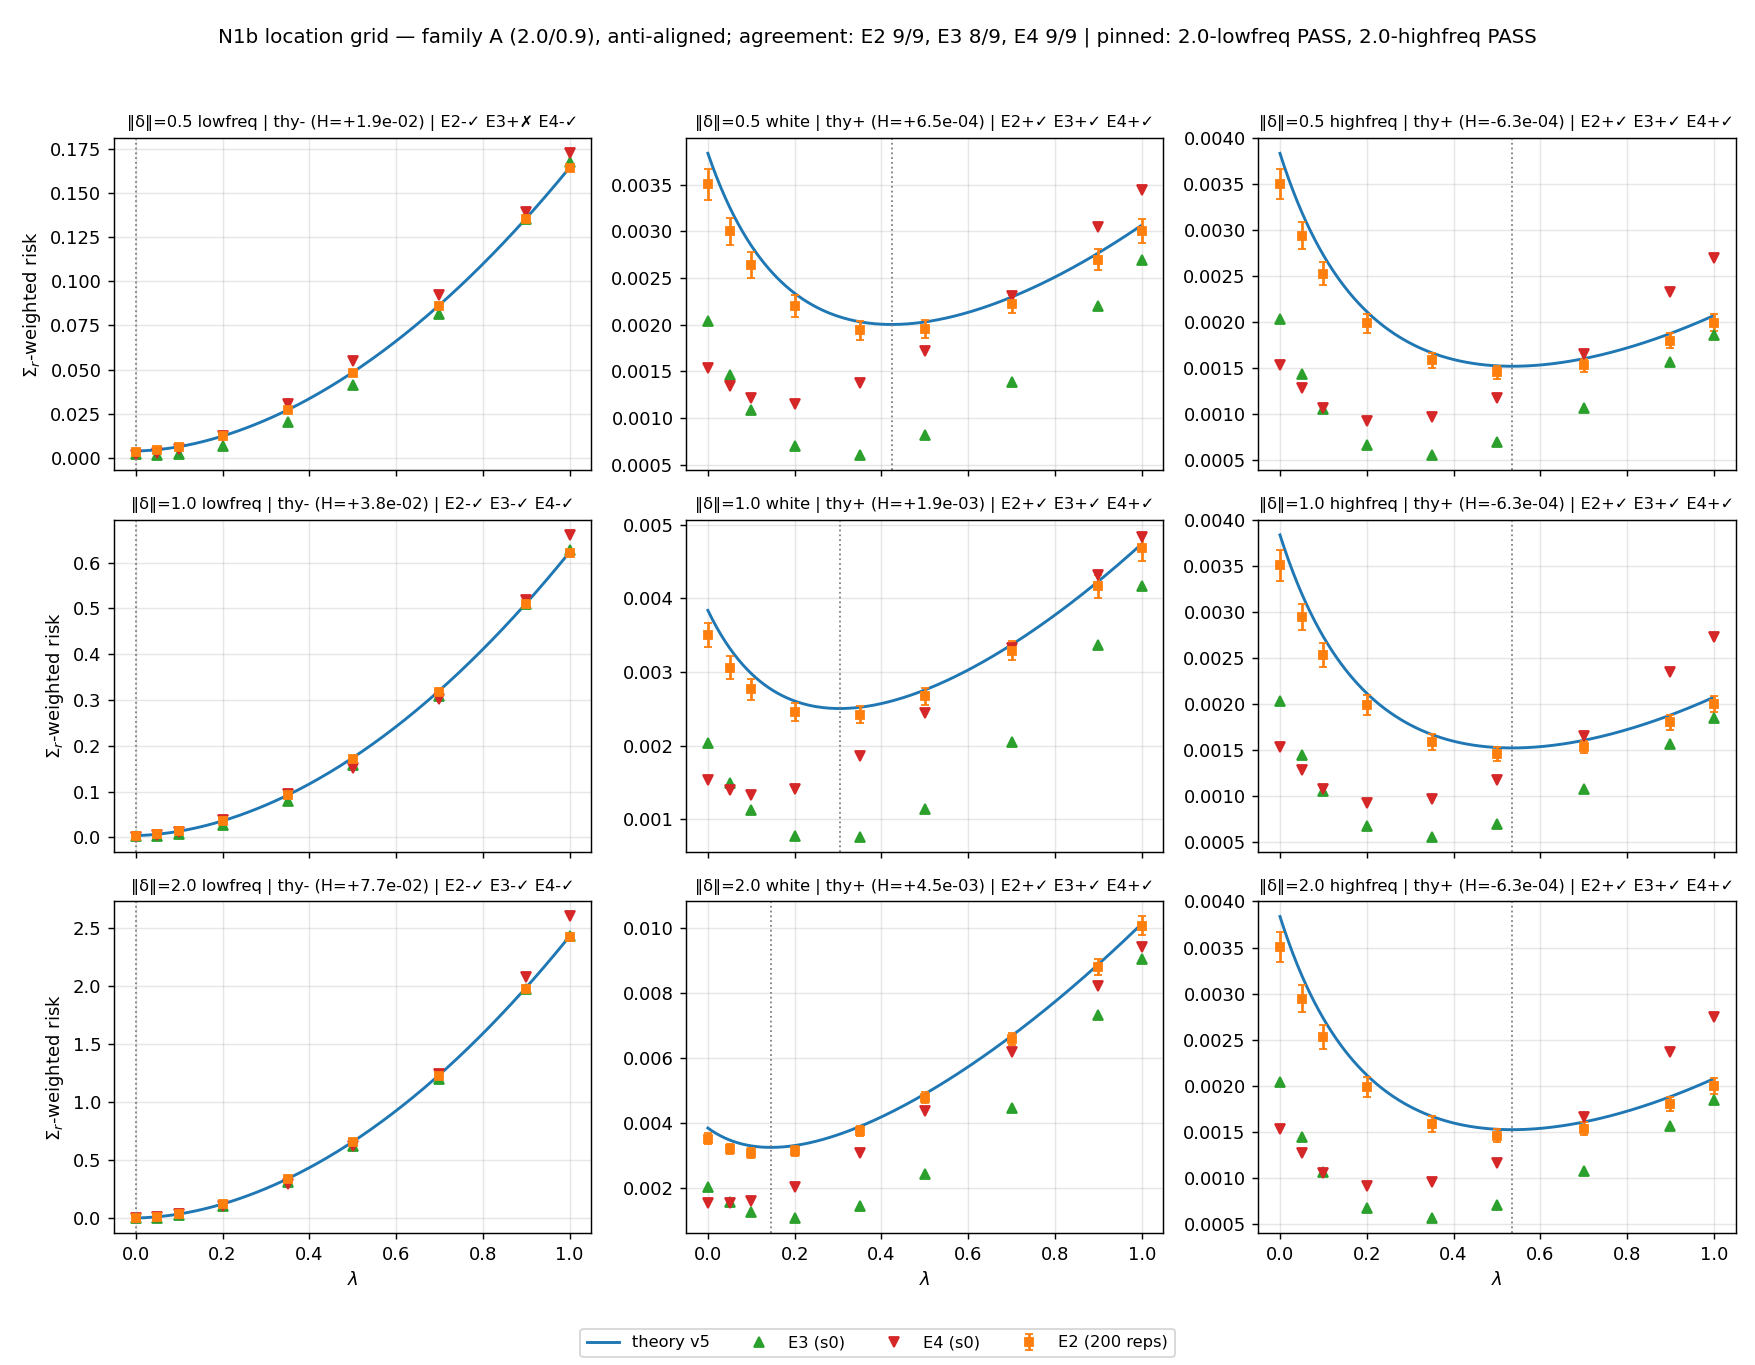
\includegraphics[width=\linewidth]{fig/n1b_location_grid.png}
  \caption{\textbf{Boundary analysis: an uncontrolled mismatch-location contrast.}
  Each cell shows target-domain excess risk versus mixing ratio $\lambda$ under anti-aligned mismatch of magnitude $\|\delta\|$ (rows) placed on low-frequency, white, or high-frequency coordinates (columns).
  Solid line: the diagonalized leading-order risk in the supplementary; markers: closed-form full ridge (200 replicates) and Adam-trained linear and MLP estimators (single seed).
  The low-versus-high-frequency contrast is strong, but location, target-weighted energy, and alignment vary together in this grid.
  A controlled candidate-family experiment with $\|\delta\|$, $\delta^\top\Sigma_r\delta$, and $c$ fixed instead finds stable amplitude variation without a sign flip of $H$.
  Sign agreement with the finite-$n_r$ criterion: 9/9 (ridge), 9/9 (MLP, exploratory single seed), 8/9 (full-batch-Adam linear, single seed). These are auxiliary observations, not evidence of an independent location-driven phase transition.}
  \label{fig:location-grid}
\end{figure*}
